\chapter{Gestione delle transazioni}

Le transazioni il paradigma utilizzato dai DBMS per gestire richieste concorrenti di lettura e scrittura sui dati.

Le transazioni sono suddivise principalmente in 3 parti:
\begin{itemize}
    \item Inizio della transazione
    \item Corpo di azioni della transazione
    \item Fine della transazione dove viene deciso se fare un commit della stessa oppure un rollback.
\end{itemize}

Un sistema transazionale è detto anche \textbf{OLTP} ed è in grado di definire ed eseguire transazioni per conto di un certo numero di applicazioni concorrenti. In parole più semplici offre un'interfaccia trasparente alle applicazioni mantenendo sicuro l'agire sui dati.

\begin{lstlisting}
start transaction;
update ContoCorrente
set Saldo = Saldo + 10 where NumConto = 12202;
update ContoCorrente
set Saldo = Saldo - 10 where NumConto = 42177;
commit work;
\end{lstlisting}

\section{ACID}

Abbiamo quindi che un'applicazione effettua molteplici transazioni e molte applicazioni effettuano parecchie transazioni in parallelo. Risulta importante per la base dati mantenere quindi il concetto di \textbf{ACID}

\textbf{ACID} é l'acronimo di:
\begin{itemize}
    \item Atomicity (Atomicità)
    \item Consistency (Consistenza)
    \item Isolation (Isolamento)
    \item Durability (Persistenza)
\end{itemize} 

Una transazione deve essere un'unità \textbf{atomica} di elaborazione. In parole semplici, o la transazione è fatta per intero oppure non deve essere eseguita per nulla.

\begin{exmp}
    L'esempio più classico di questa proprietà è quando si fa un movimento monetario in banca.
    
    Quando devo muovere del denaro da un conto ad un altro dovrò rimuovere del denaro da un primo conto e aggiungerlo in un secondo conto. Se per qualche malaugurato caso l'operazione non andasse a buon fine in un momento intermedio si rischierebbe di sballare i conteggi di uno dei due conti se non di entrambi.
    
    Cosa che per una banca può essere un problema di migliaia o milioni di euro.
\end{exmp}

Una transazione deve essere \textbf{Consistente}, deve infatti rispettare i vincoli imposti nella fase di progettazione del Database, come chiave, integrità referenziale, check, ecc.

Questi vincoli che determinano la consistenza dei dati vanno verificati solo a fine transazione, possono quindi essere violati temporaneamente nel mezzo di una transazione.

Se i vincoli risultano violati alla fine della transazione allora la transazione andrà in rollback.

Una transazione deve essere poi \textbf{Isolata}, non deve infatti risentire degli effetti delle altre transazioni concorrenti. In poche parole l'esecuzione concorrente deve produrre un risultato identico a quello che verrebbe ottenuto se le transazioni concorrenti venissero invece eseguite sequenzialmente.

Se una transazione esponesse i suoi stati intermedi si rischierebbe un effetto domino.

Gli effetti di una transazione che ha raggiunto il commit non devono essere persi in qualsiasi csao, anche in presenza di guasti.

Sia che questi guasti siano di dispositivo\footnote{Hardware} oppure che questi guasti siano di sistema\footnote{Software}.

\section{Processi di ripresa}

Le riprese da un crash sono di due tipi: ripresa a caldo e ripresa a freddo.

Una ripresa a freddo viene eseguita quando il problema è stato a livello Hardware, in quel caso si deve ripristinare i dati da un dump e in secondo luogo eseguire la ripresa a caldo.

La ripresa a caldo risolve tutti i problemi relativi alle transazioni in atto al momento del crash.

La ripresa a freddo si avvale di un dump eseguito periodicamente nel log. Il dump in oggetto viene copiato nel database e ne ripristina i dati fino al suo momento.

Dopo il dump bisognerà invece scorrere il log ed eseguire tutte le transazioni nella sequenza indicata.

\section{I vari schedule}

Uno schedule è una sequenza di operazioni di input/output concorrenti.

Lo \textbf{scheduler} invece è il sistema che accetta, rifiuta o riordina le operazioni richieste dalle transazioni.

Esistono vari tipi di \textbf{Scheduling} che ritornano vari tipi di schedule.

In uno schedule seriale le transazioni sono seprate e vengono eseguite una alla volta, questo tipo di schedule è sicuro perché eseguendo tutte le operazioni in ordine non è possibile trovarsi in una situazione di race condition. In tutti gli schedule successivi si cercherà infatti di tornare a questo tipo di schedule.

Avremo infatti uno \textbf{schedule serializzabile} quando uno schedule produce lo stesso risultato di uno schedule seriale eseguito sulle stesse transazioni.

\[ \text{Schedule seriale} \implies \text{Schedule serializzabile}\]

L'insieme degli schedule serializzabili contiene l'insieme degli schedule seriali.

Gli schedule serializzabili utilizzati sono:
\begin{itemize}
    \item View serializzabili
    \item Conflict serializzabili
    \item Two Phase locking
\end{itemize}

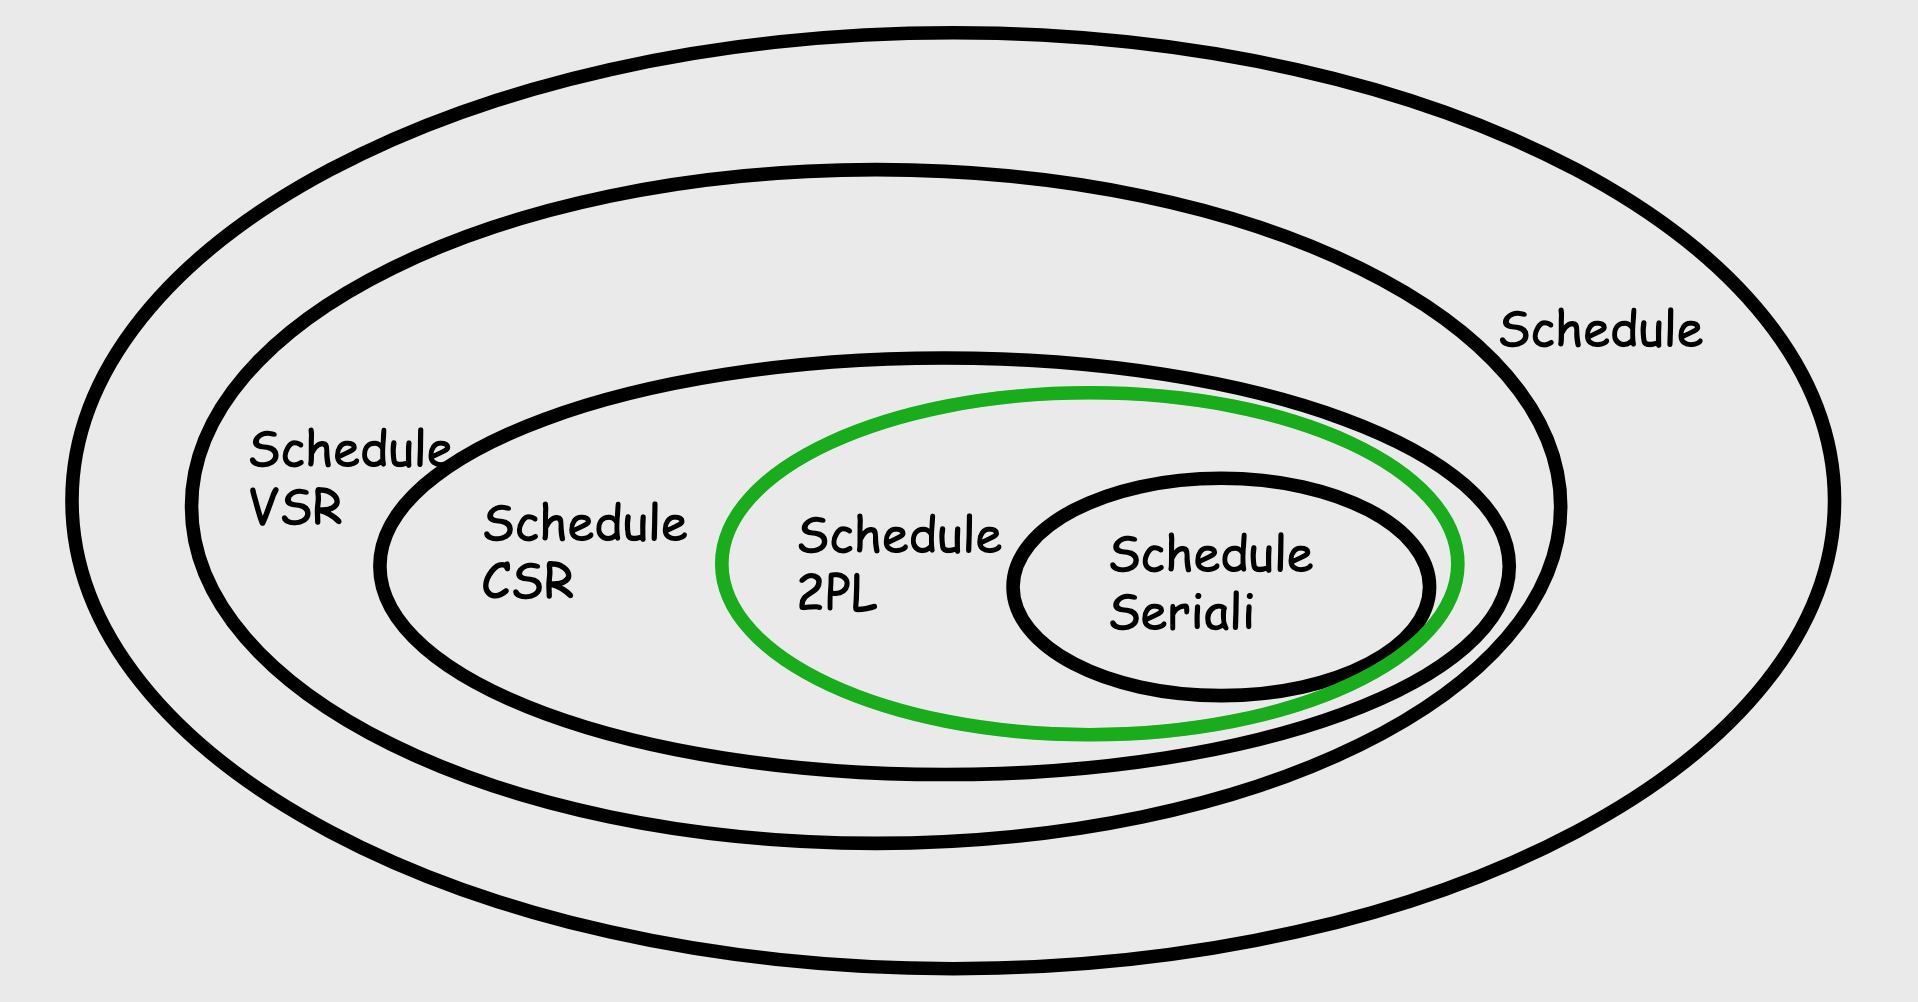
\includegraphics[width=\linewidth]{img/schedules.png}

\subsection{View serializzabilità}

Uno schedule è view serializzabile se è view equivalente ad almeno uno schedule seriale.

Uno schedule è view equivalente ad un altro se le letture leggono dagli stessi eventi come nell'altro schedule e la sequenza di scritture finali è la stessa.

Uno schedule view serializzabile offre numerose \textbf{garanzie}
\begin{itemize}
    \item Assienza di perdita di aggiornamento
    \item Assenza di letture inconsistenti
    \item Assenza di Gost updates
\end{itemize}

\subsection{Conflict serializzabilità}

Siccome cercare la view serializzabilità con molte transazioni diventa un lavoro molto costoso, si preferisce cercare la conflict serializzabilità. Si ha infatti che costa meno in tempo eseguire serialmente uno schedule view serializzabile ma non conflict serializzabile piuttosto che conoscere se esso è view serializzabile oppure no.

Se uno schedule è Conflict serializzabile allora è sicuramente anche View serializzabile. Uno schedule Conflict serializzabile è un sottoinsieme degli schedule View serializzabili.

\[CSR \implies VSR \implies \text{Schedule serializzabile}\]

Se uno schedule è conflict serializzabile allora è possibile costruire un grafo aciclico dei conflitti.

Infatti se abbiamo un grafo aciclico dei conflitti possiamo anche comprendere se il nostro schedule è conflict serializzabile. Inoltre il grafo ci può fornire anche un ordine in cui le transazioni devono essere eseguite per avere uno schedule seriale.

Lo schedule seriale è conflict equivalente e quindi view equivalente. Ovvero posso trovare uno schedule conflict serializzabile, conflict equivalente ad uno schedule seriale.

\subsection{Svolgere gli esercizi}

\begin{exmp}
    Data lo schedule:

    \[S = r_1(x), w_2(x), r_3(x), w_1(u), w_3(v), r_3(y), r_2(y), w_3(u), w_4(t), w_3(t)\]

    Possiamo dire se è conflict serializzabile disegnando il grafo dei conflitti.

    Seguendo l'algoritmo scorriamo ognuno dei punti della serie di transazioni e vediamo se va in conflitto con una qualsiasi altra unità di transazione.

    Ad esempio, partendo da \textbf{$r_1$} che fa una lettura su \textbf{$x$}, vediamo che la stessa \textbf{$x$} è utilizzata in \textbf{$w_2$}. \textbf{$r_3$} non è in conflitto con \textbf{$r_1$} in quanto essendo due letture non ho problemi anche se l'accesso fosse simmultaneo.

    Disegnamo allora un vettore da dalla transazione 1 alla transazione 2.
    \begin{center}
        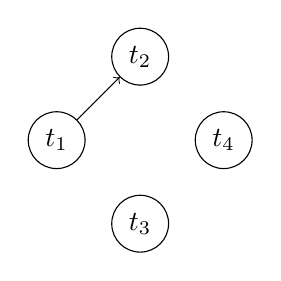
\begin{tikzpicture}[node distance={15mm}, main/.style = {draw, circle}] 
        
            \node[main] (1) {$t_1$}; 
            \node[main] (2) [above right of=1]{$t_2$}; 
            \node[main] (3) [below right of=1]{$t_3$}; 
            \node[main] (4) [above right of=3]{$t_4$};
            \draw[->] (1) -- (2);
        \end{tikzpicture} 
    \end{center}

    Continuando a seguire l'algoritmo per tutti gli altri punti il risultato è il seguente:
    \begin{center}
        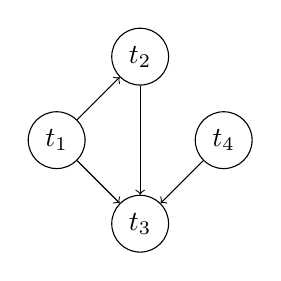
\begin{tikzpicture}[node distance={15mm}, main/.style = {draw, circle}] 
        
            \node[main] (1) {$t_1$}; 
            \node[main] (2) [above right of=1]{$t_2$}; 
            \node[main] (3) [below right of=1]{$t_3$}; 
            \node[main] (4) [above right of=3]{$t_4$};
            \draw[->] (1) -- (2);
            \draw[->] (2) -- (3);
            \draw[->] (1) -- (3);
            \draw[->] (4) -- (3);
        \end{tikzpicture} 
    \end{center}

    Da questo grafo appena disegnato possiamo quindi estrarre uno Schedule seriale.

    Per prima cosa andranno tutte le transazioni senza vertici entranti, ovvero $t_1, t_4$ dopo questo l'algoritmo continua contando i nodi già estratti come senza vertici uscenti.

    Il risultato è quindi la sequenza $t_1 \rightarrow t_4 \rightarrow t_2 \rightarrow t_3$.
    
    Lo schedule seriale è quindi:

    
    \begin{center}
        \begin{tabularx}{10cm}{|p{25mm}|X|}
            \hline
            \rowcolor{gray!30}
            \textbf{Transazione} & \textbf{operazioni}\\
            \hline
            $t_1$& $r_1(x), w_1(u)$\\
            $t_4$& $w_4(t)$\\
            $t_2$& $w_2(x), r_2(y)$\\
            $t_3$& $r_3(x), w_3(v), r_3(y), w_3(u), w_3(t)$\\
            \hline
        \end{tabularx}
    \end{center}

    Che risulta nello schedule completo:
    \[S_\text{seriale} = r_1(x), w_1(u), w_4(t), w_2(x), r_2(y), r_3(x), w_3(v), r_3(y), w_3(u), w_3(t)\]
\end{exmp}
